\section{Empirical Evaluation}

In this section, we present the performance of \model through two primary methods: \textit{automated metric evaluation} and \textit{human assessment}. %, providing a thorough analysis of the performance and quality of the generated videos. 
We train the \model models with different parameter sizes. 
We show results for 2B and 5B for now, larger models are still in training.
% The following evaluation defaults to using our largest model to date, which can also be accessed via the website \url{https://ChatGLM.cn} or via APIs at \url{https://bigmodel.cn}. 

To facilitate the development of text-to-video generation, we open-source the model weight at \url{https://github.com/THUDM/CogVideo}.

%We trained a series of models of various sizes. For all subsequent evaluations, we will use the largest model (referred to as CogVideoX). 


\subsection{Automated Metric Evaluation} 

\paragraph{Baselines.} 
We choose openly-accessible top-performing text-to-video models as baselines, including T2V-Turbo~\citep{li2024t2v}, AnimateDiff~\citep{guo2023animatediff}, VideoCrafter2~\citep{chen2024videocrafter2}, OpenSora~\citep{opensora}, Show-1~\citep{zhang2023show}, Gen-2~\citep{gen2}, Pika~\citep{pika}, and LaVie-2~\citep{wang2023lavie}.



\begin{table}[t]
\caption{Evaluation results.}
\label{table:results}
\vspace{6pt}
\footnotesize
    \centering
    \begin{tabular}{cccccccc}
   \toprule
        Models & \Centerstack{Human \\Action}   & Scene & \Centerstack{Dynamic \\Degree} & \Centerstack{Multiple \\Objects} & \Centerstack{Appearance \\Style} & \Centerstack{Dynamic \\Quality} & \Centerstack{GPT4o-MT \\Score}  \\ 
        \midrule
        T2V-Turbo & 95.2 & \textbf{55.58} & 49.17 & 54.65 & 24.42 & -- & --  \\ 
        AnimateDiff & 92.6  & 50.19 & 40.83 & 36.88 & 22.42 & -- & 2.62  \\ 
        VideoCrafter-2.0 & 95.0  & 55.29 & 42.50 & 40.66 & \textbf{25.13} & 43.6 & 2.68  \\ 
        OpenSora V1.2 & 85.8  & 42.47 & 47.22 & 58.41  & 23.89 & 63.7 & 2.52  \\ 
        Show-1 & 95.6  & 47.03 & 44.44 & 45.47  & 23.06 & 57.7 & --  \\ 
        Gen-2 & 89.2  & 48.91 & 18.89 & 55.47 & 19.34 & 43.6 & 2.62  \\ 
        Pika & 88.0  & 44.80 & 37.22 & 46.69  & 21.89 & 52.1 & 2.48  \\ 
        LaVie-2 & 96.4 & 49.59 & 31.11 & 64.88  & 25.09 & -- & 2.46  \\ 
        \hline
        \textbf{CogVideoX-2B} & 88.0 & 39.94 & \textbf{63.33} & 53.70 & 23.67 & 57.7 & 3.09 \\
        \textbf{CogVideoX-5B} & \textbf{96.8} & 55.44 & 62.22 & \textbf{70.95} & 24.44 & \textbf{69.5} & \textbf{3.36} \\
        \bottomrule
    \end{tabular}
\end{table}

\paragraph{Evaluation Metrics.} 
To evaluate the text-to-video generation, we employed several metrics from VBench~\citep{huang2023vbench}: \emph{Human Action}, \emph{Scene}, \emph{Dynamic Degree}, \emph{Multiple Objects}, and \emph{Appearance Style}. 
VBench is a suite of tools designed to automatically assess the quality of generated videos. We have selected certain metrics from VBench, excluding others that do not align with our evaluation needs. 
For example, the color metric, intended to measure the presence of objects corresponding to specific colors across frames in the generated video, assesses the model's quality by calculating the probability. 
However, this metric may mislead video generation models that exhibit greater variation, thus it is not to include it in our evaluation. 

For longer-generated videos, some models might produce videos with minimal changes between frames to obtain higher scores, but these videos lack rich content. 
Therefore, a metric for evaluating the dynamism of the video becomes more important. 
To address this, we employ two video evaluation tools:  \emph{Dynamic Quality} from Devil~\citep{liao2024evaluationtexttovideogenerationmodels} and \emph{GPT4o-MTScore} from ChronoMagic~\citep{yuan2024chronomagic}, which focus more on the dynamic characteristics of videos. 
\emph{Dynamic Quality} is defined by the integration of various quality metrics with dynamic scores, mitigating biases arising from negative correlations between video dynamics and video quality.
%leading to a more thorough assessment of video quality. 
ChronoMagic, for instance, introduces {GPT4o-MTScore}, a metric designed to measure the metamorphic amplitude of time-lapse videos, such as those depicting physical, biological, and meteorological changes. 
This metric using GPT-4o~\citep{gpt4o} to score the degree of change, providing a fine-grained assessment of video dynamism. 
%is obtained by extracting frames from the generated videos at regular intervals and using GPT-4o~\citep{gpt4o} to score the degree of change, providing a fine-grained assessment of video dynamism. 
% This method ensures a more accurate evaluation of the content's variability over time, countering the potential bias of static frame sequences in scoring.



\paragraph{Results.} 
Table~\ref{table:results} provides the performance comparison of \model and other models. 
\model achieves the best performance in five out of the seven metrics and shows competitive results in the remaining two metrics. 
These results demonstrate that the model not only excels in video generation quality but also outperforms previous models in handling various complex dynamic scenes. 
In addition, Figure~\ref{fig:radar} presents a radar chart that visually illustrates the performance advantages of \model.


\begin{figure}[ht]
\begin{center}
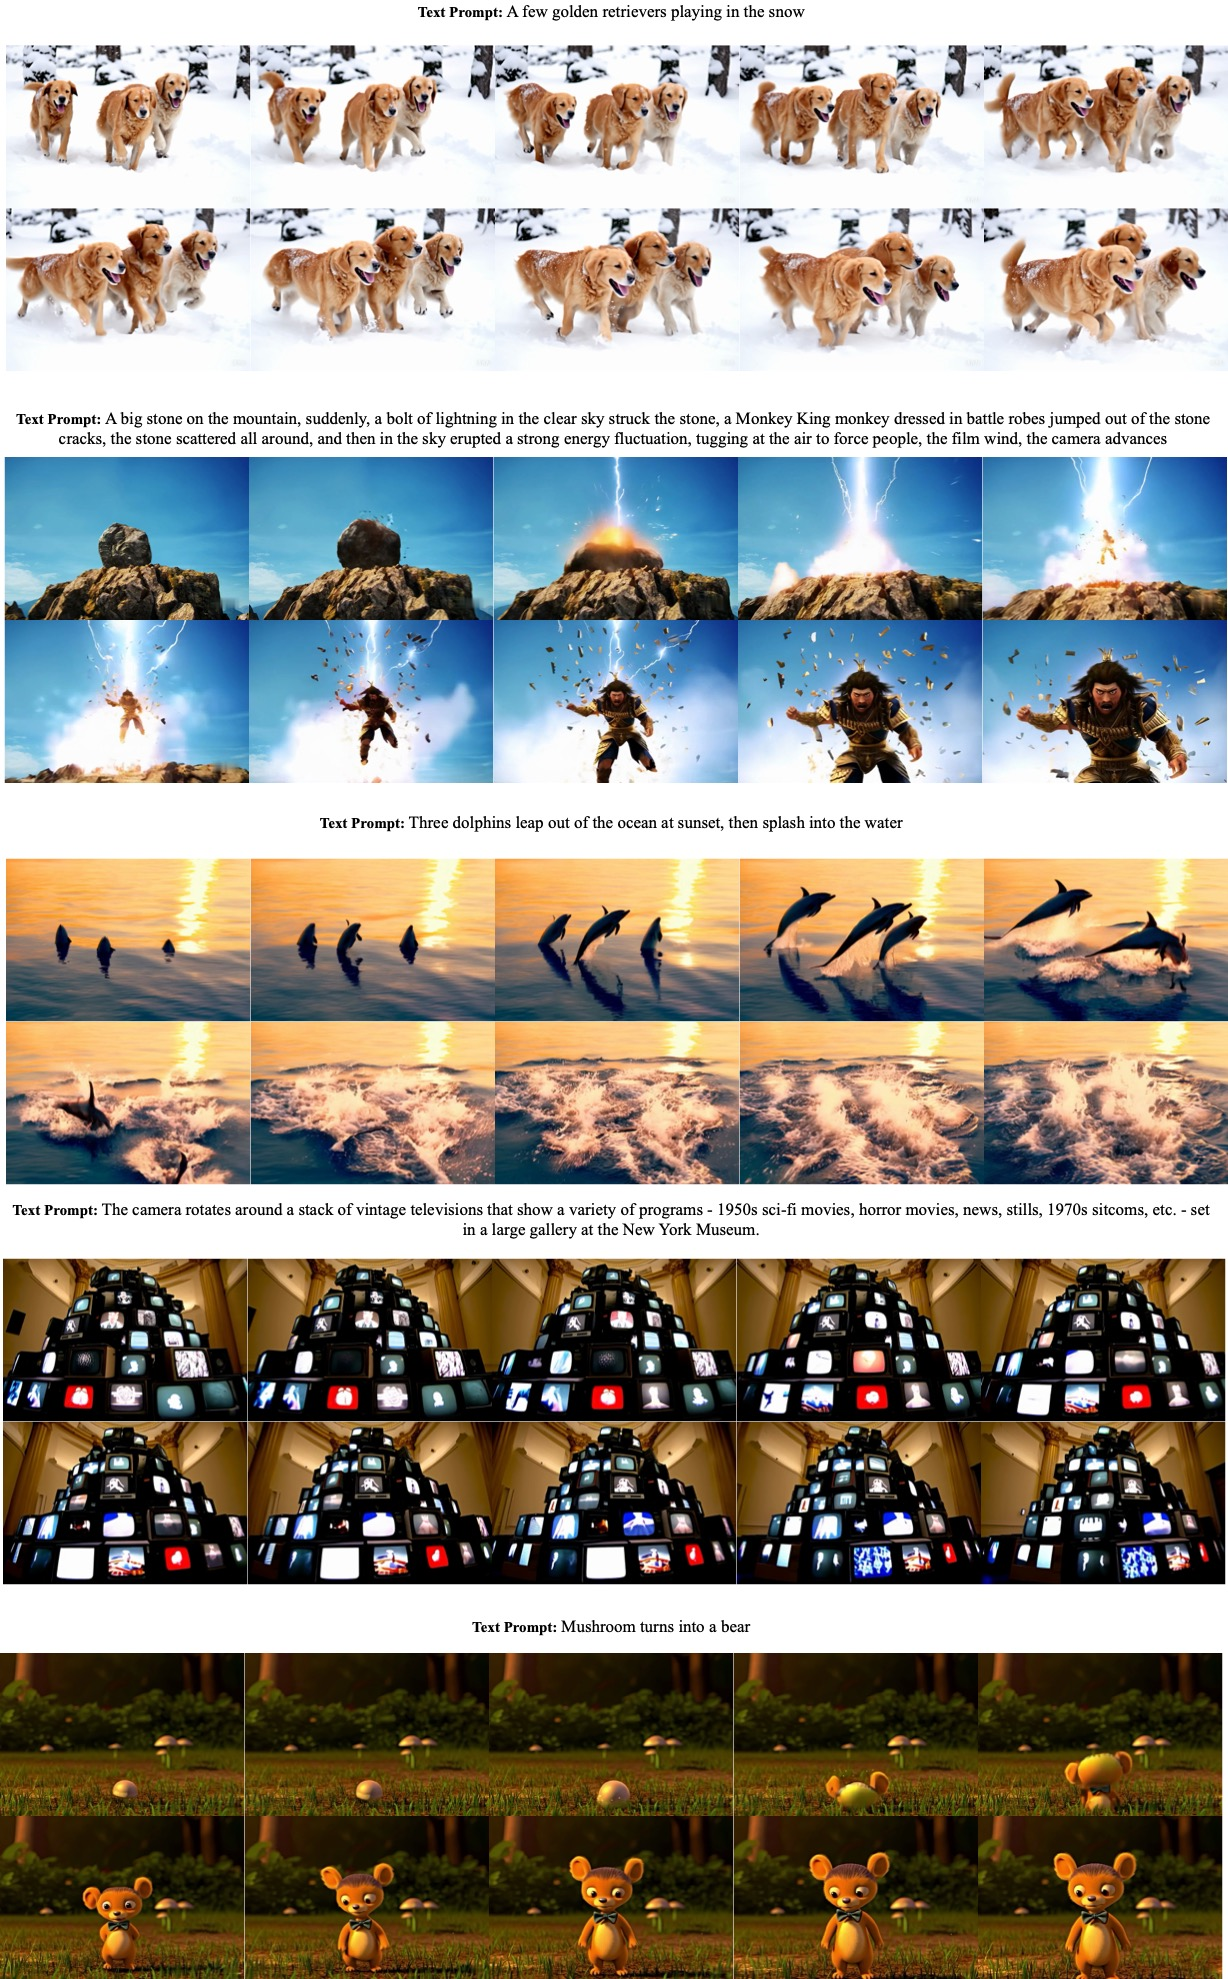
\includegraphics[width=\linewidth]{images/t2v/goodcase1.jpg}
\end{center}
\caption{Text to video showcases. The displayed prompt will be upsampled before being fed into the model. The generated videos contain large motion and can produce various video styles.}
\label{fig:t2vgood1}
\end{figure}

\begin{figure}[ht]
\begin{center}
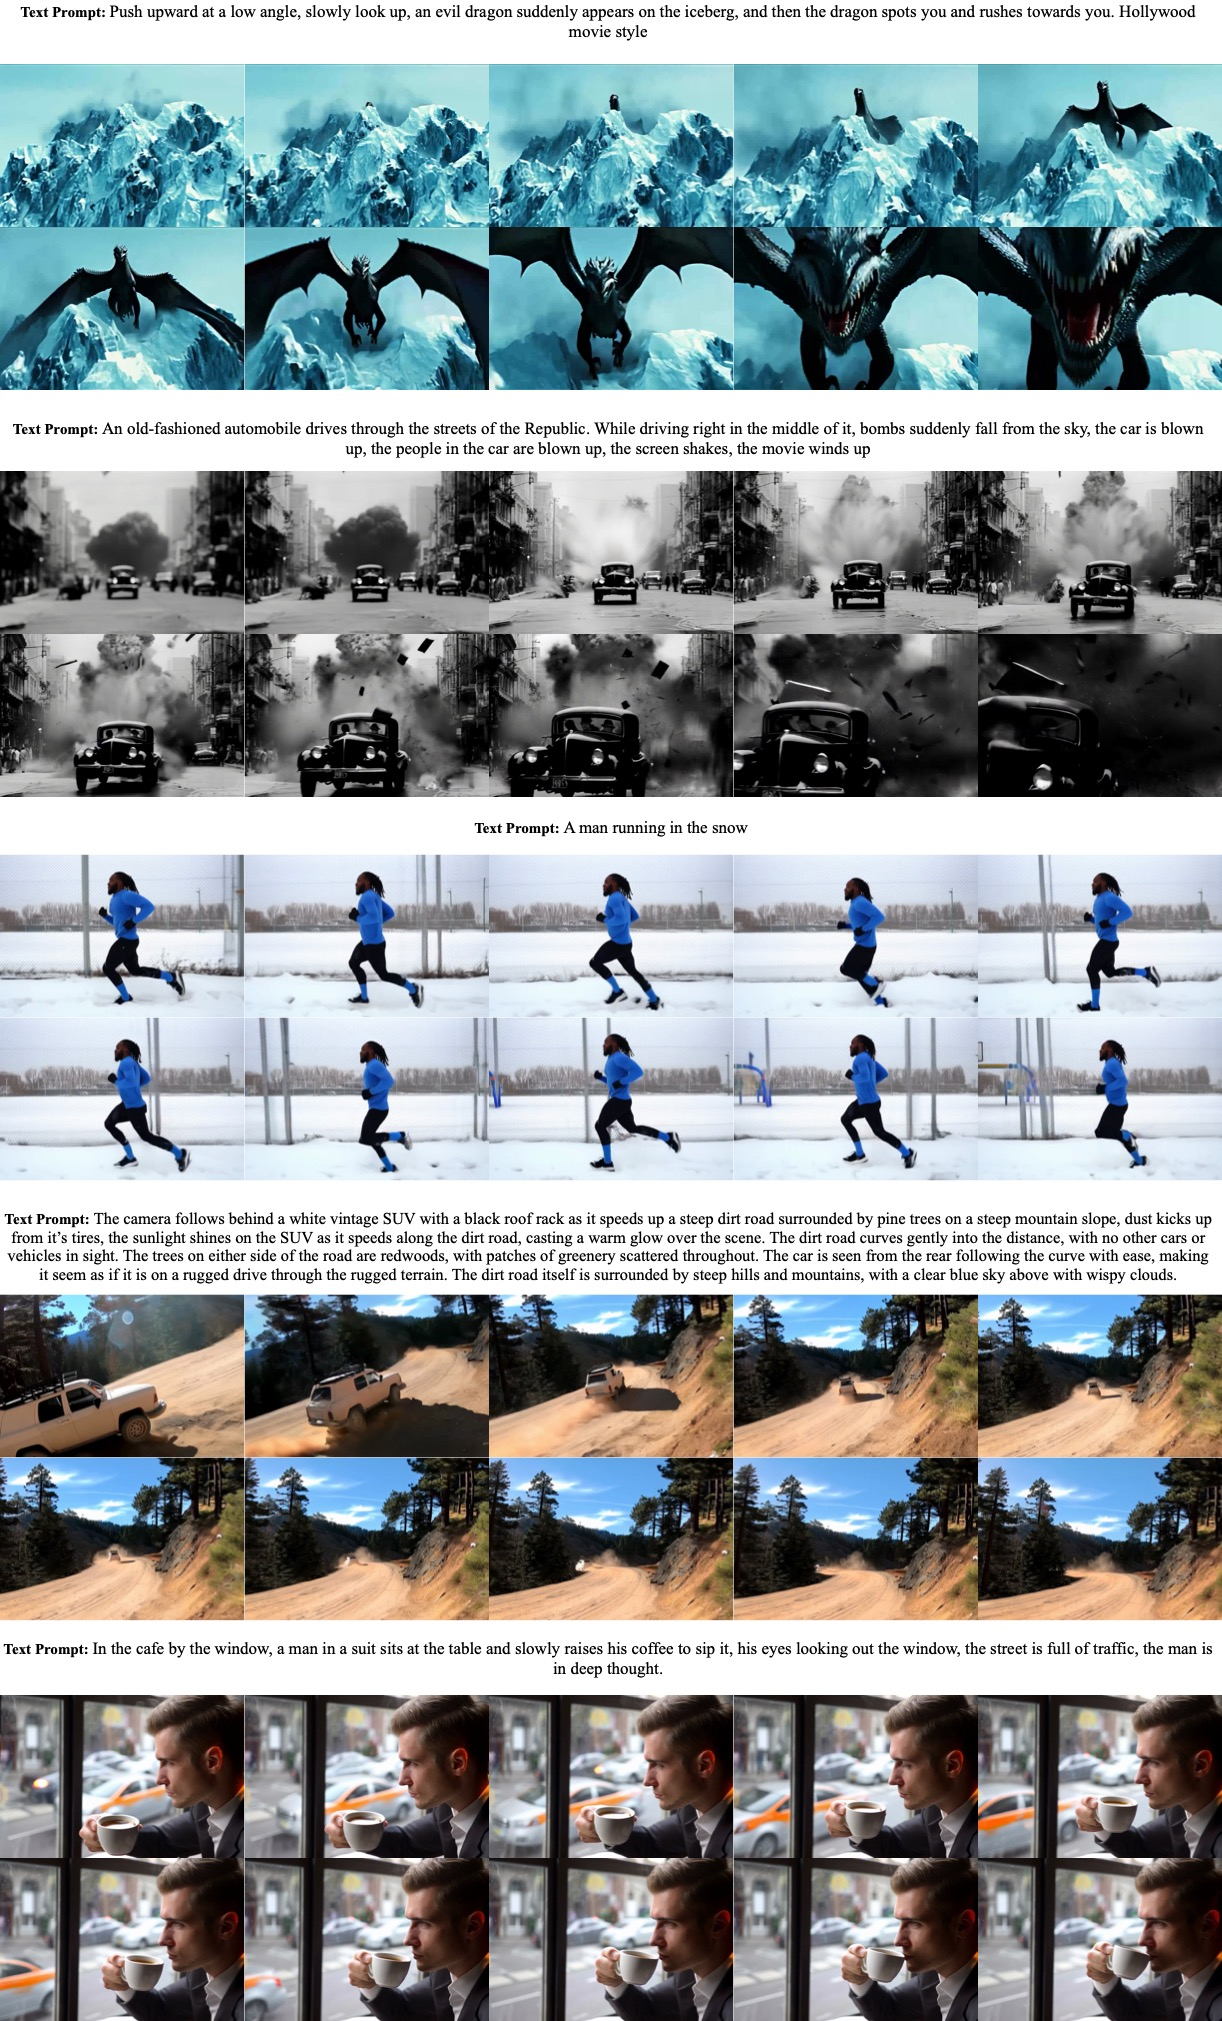
\includegraphics[width=0.98\linewidth]{images/t2v/goodcase2.jpg}
\end{center}
\caption{Text to video showcases.}
\label{fig:t2vgood2}
\end{figure}


% Please add the following required packages to your document preamble:
% \usepackage[table,xcdraw]{xcolor}
% Beamer presentation requires \usepackage{colortbl} instead of \usepackage[table,xcdraw]{xcolor}
% \usepackage[normalem]{ulem}
% \useunder{\uline}{\ul}{}




% \begin{table}[]

% \centering
% \setlength\tabcolsep{3pt}

% \label{sample-table}
% \small
% \vspace{-10pt}
% \caption{\textbf{Automatic Evaluation Results per Dimension.}The table presents a comparative analysis of various video models across different dimensions. It is evident from the table that, in terms of both human motion and background effects as well as the accuracy and distinctiveness of objects, CogVideoX has achieved the current SOTA level. Furthermore, CogVideoX has garnered a commendable score in the expression of dynamic qualities, a capability that serves as a more precise indicator of the intrinsic properties of video media, distinct from the static nature of photographic images.}

% \vspace{6pt}

% \begin{tabular}{cccccccc}
% \toprule
% \multirow{2}{*}{\textbf{Models} }  & \textbf{human}  & \textbf{object} &\multirow{2}{*}{\textbf{scene}}&\textbf{dynamic} &\textbf{multiple} &\textbf{spatial} &\textbf{appearance} \\
%     & \textbf{action}& \textbf{class}& & \textbf{degree} &\textbf{objects}& \textbf{relationship}&\textbf{style}  
% \\
% \midrule
% CogVideoX & 96.80\% &93.70\% & 55.44\% & 62.22\% & 70.95\% & 61.29\% & 24.44\% \\
% {LaVie-2} & 96.40\% & 97.52\%  & 49.59\% & 31.11\% & 64.88\%  & 38.68\% & 25.09\%  \\
% {T2V-Turbo}  & 95.20\%  & 93.96\%& 55.58\% & 49.17\% & 54.65\%    & 38.67\%  & 24.42\%   \\
% {Gen-2}  & 89.20\%& 90.92\%  & 48.91\%  & 18.89\% & 55.47\%    & 66.91\%   & 19.34\%  \\
% {VideoCrafter-2.0\citep{chen2024videocrafter2}} & 95.00\% & 92.55\% & 55.29\%               & 42.50\% & 40.66\% & 35.86\% & 25.13\%  \\
% {Pika Beta} & 88.00\% & 87.45\%  & 44.80\% & 37.22\% & 46.69\% & 65.65\% & 21.89\%   \\
% AnimateDiff-V2 & 92.60\% & 90.90\%  & 50.19\% & 40.83\%        & 36.88\% & 34.60\%  & 22.42\%\\
% {OpenSora V1.2}   & 85.80\% & 83.37\%& 42.47\%   & 47.22\%    & 58.41\% & 67.51\%  & 23.89\%  \\
% {Show-1} & 95.60\%  & 93.07\%  & 47.03\% & 44.44\% & 45.47\% & 53.50\%  & 23.06\%  \\
% {HiGen}  & 86.20\%  & 86.06\%  & 44.88\% & 99.17\% & 22.39\%  & 22.43\% & 24.54\% \\  
% \bottomrule
% \end{tabular}
% \end{table}



% \iffalse



% \begin{table}[ht!]
% \centering
% \caption{Evaluation results.}
% \setlength\tabcolsep{3pt}
% \label{sample-table}
% \begin{center}
% \small
% \resizebox{0.9\linewidth}{!}{
% \begin{tabular}{ccccccccc}

% \multirow{2}{*}{\textbf{Models} }  & \textbf{subject}  & \textbf{background} &\textbf{temporal} &\textbf{motion} &\textbf{dynamic} &\textbf{aesthetic} &\textbf{imaging} &\textbf{object} \\
%     & \textbf{consistency}& \textbf{consistency}& \textbf{flickering}& \textbf{smoothness} &\textbf{degree}& \textbf{quality}&\textbf{quality} & \textbf{class}
% \\ \hline 
%         CogVideoX & 94.66\% & 95.92\% & 97.47\% & 98.10\% & 62.22\% & 55.14\% & 63.62\% & 93.70\%  \\
%         LaVie-2 & 97.90\% & 98.45\% & 98.76\% & 98.42\% & 31.11\% & 67.62\% & 70.39\% & 97.52\%  \\ 
%         T2V-Turbo (VC2) & 96.28\% & 97.02\% & 97.48\% & 97.34\% & 49.17\% & 63.04\% & 72.49\% & 93.96\%  \\ 
%         Gen-2 (2023-06) & 97.61\% & 97.61\% & 99.56\% & 99.58\% & 18.89\% & 66.96\% & 67.42\% & 90.92\%  \\ 
%         VideoCrafter-2.0\citep{chen2024videocrafter2} & 96.85\% & 98.22\% & 98.41\% & 97.73\% & 42.50\% & 63.13\% & 67.22\% & 92.55\%  \\ 
%         Pika Beta (2023-06) & 96.76\% & 98.95\% & 99.77\% & 99.51\% & 37.22\% & 63.15\% & 62.33\% & 87.45\%  \\ 
%         AnimateDiff-V2 & 95.30\% & 97.68\% & 98.75\% & 97.76\% & 40.83\% & 67.16\% & 70.10\% & 90.90\%  \\ 
%         OpenSora V1.2 & 94.45\% & 97.90\% & 99.47\% & 98.20\% & 47.22\% & 56.18\% & 60.94\% & 83.37\%  \\ 
%         Show-1 & 95.53\% & 98.02\% & 99.12\% & 98.24\% & 44.44\% & 57.35\% & 58.66\% & 93.07\%  \\ 
%         HiGen & 90.07\% & 93.99\% & 93.24\% & 96.69\% & 99.17\% & 57.30\% & 63.92\% & 86.06\% \\ 
% \hline \\

% \multirow{2}{*}{\textbf{Models} }  & \textbf{multiple}  & \textbf{human} &\multirow{2}{*}{\textbf{color}} &\textbf{spatial} &\multirow{2}{*}{\textbf{scene}} &\textbf{appearance} &\textbf{temporal} &\textbf{overall} \\
%     & \textbf{objects}& \textbf{action}& & \textbf{relation} & & \textbf{style}&\textbf{style} & \textbf{consistency}
% \\ \hline 
%         CogVideoX & 70.95\% & 96.80\% & 79.75\% & 61.29\% & 55.44\% & 24.44\% & 23.69\% & 26.73\%  \\ 
%         LaVie-2 & 64.88\% & 96.40\% & 91.65\% & 38.68\% & 49.59\% & 25.09\% & 25.24\% & 27.39\%  \\ 
%         T2V-Turbo (VC2) & 54.65\% & 95.20\% & 89.90\% & 38.67\% & 55.58\% & 24.42\% & 25.51\% & 28.16\%  \\
%         Gen-2 (2023-06) & 55.47\% & 89.20\% & 89.49\% & 66.91\% & 48.91\% & 19.34\% & 24.12\% & 26.17\%  \\ 
%         VideoCrafter-2.0 & 40.66\% & 95.00\% & 92.92\% & 35.86\% & 55.29\% & 25.13\% & 25.84\% & 28.23\%  \\
%         Pika Beta (2023-06) & 46.69\% & 88.00\% & 85.31\% & 65.65\% & 44.80\% & 21.89\% & 24.44\% & 25.47\%  \\ 
%         AnimateDiff-V2 & 36.88\% & 92.60\% & 87.47\% & 34.60\% & 50.19\% & 22.42\% & 26.03\% & 27.04\%  \\ 
%         OpenSora V1.2 & 58.41\% & 85.80\% & 87.49\% & 67.51\% & 42.47\% & 23.89\% & 24.55\% & 27.07\%  \\ 
%         Show-1 & 45.47\% & 95.60\% & 86.35\% & 53.50\% & 47.03\% & 23.06\% & 25.28\% & 27.46\%  \\ 
%         HiGen & 22.39\% & 86.20\% & 86.22\% & 22.43\% & 44.88\% & 24.54\% & 25.14\% & 27.14\% \\ \hline

% \hline \\
% \end{tabular}

% }
% \end{center}
% \end{table}

% \fi






% \begin{table}[!ht]
% \centering

% \label{sample-table}
% \small
% \vspace{-10pt}
% \caption{\textbf{Automatic Evaluation Results per Dimension.}}

% \vspace{6pt}

% \resizebox{0.8\linewidth}{!}{
%     \begin{tabular}{cccc}
%         \textbf{Models} & \textbf{\Centerstack{Dynamics Range}} & \textbf{\Centerstack{Dynamics Controllability}} & \textbf{\Centerstack{Dynamics-based Quality}} \\ \hline
%         CogVideoX       & 55.7 & 71.8 & \textbf{69.5} \\ 
%         Gen-2           & 30.8 & \textbf{82.5} & 43.6 \\ 
%         Pika            & 43.2 & 72.0 & 52.1 \\ 
%         VideoCrafter2   & 34.1 & 57.0 & 43.6 \\ 
%         OpenSora        & \textbf{61.2} & 62.4 & 63.7 \\ 
%         Show-1          & 45.1 & 73.9 & 57.7 \\ 
%     \end{tabular}
% }
% \end{table}



\begin{table}[t]
\caption{Evaluation results.}
\label{table:results}
\vspace{6pt}
\footnotesize
    \centering
    \begin{tabular}{cccccccc}
   \toprule
        Models & \Centerstack{Human \\Action}   & Scene & \Centerstack{Dynamic \\Degree} & \Centerstack{Multiple \\Objects} & \Centerstack{Appearance \\Style} & \Centerstack{Dynamic \\Quality} & \Centerstack{GPT4o-MT \\Score}  \\ 
        \midrule
        T2V-Turbo & 95.2 & \textbf{55.58} & 49.17 & 54.65 & 24.42 & -- & --  \\ 
        AnimateDiff & 92.6  & 50.19 & 40.83 & 36.88 & 22.42 & -- & 2.62  \\ 
        VideoCrafter-2.0 & 95.0  & 55.29 & 42.50 & 40.66 & \textbf{25.13} & 43.6 & 2.68  \\ 
        OpenSora V1.2 & 85.8  & 42.47 & 47.22 & 58.41  & 23.89 & 63.7 & 2.52  \\ 
        Show-1 & 95.6  & 47.03 & 44.44 & 45.47  & 23.06 & 57.7 & --  \\ 
        Gen-2 & 89.2  & 48.91 & 18.89 & 55.47 & 19.34 & 43.6 & 2.62  \\ 
        Pika & 88.0  & 44.80 & 37.22 & 46.69  & 21.89 & 52.1 & 2.48  \\ 
        LaVie-2 & 96.4 & 49.59 & 31.11 & 64.88  & 25.09 & -- & 2.46  \\ 
        \hline
        \textbf{CogVideoX-2B} & 88.0 & 39.94 & \textbf{63.33} & 53.70 & 23.67 & 57.7 & 3.09 \\
        \textbf{CogVideoX-5B} & \textbf{96.8} & 55.44 & 62.22 & \textbf{70.95} & 24.44 & \textbf{69.5} & \textbf{3.36} \\
        \bottomrule
    \end{tabular}
\end{table}


\subsection{Human Evaluation}
In addition to automated scoring mechanisms, a comparative analysis between the Kling~\citep{kling} and CogVideoX is conducted with manual evaluation. 
One hundred meticulously crafted prompts are used for human evaluators, characterized by their broad distribution, clear articulation, and well-defined conceptual scope. 
We randomize videos for blind evalution. 
A panel of evaluators is instructed to assign scores for each detail on a scale from zero to one, with the overall total score rated on a scale from $0$ to $5$, where higher scores reflect better video quality. 
To better complement automated evaluation, human evaluation emphasizes the instruction-following capability: the total score cannot exceed $2$ if the generated video fails to follow the instruction.

The results shown in Table~\ref{table:human_eva} indicate that \model wins the human preference over Kling across all aspects. 
More details about human evaluation are shown in Appendix~\ref{sec:human_evalution}.

\begin{table}[!ht]
\centering
\label{sample-table}
\small
\vspace{-5pt}
\caption{Human evaluation between CogVideoX and Kling.}
\label{table:human_eva}
\resizebox{0.75\linewidth}{!}{
    \begin{tabular}{cccccc}
    \toprule
        Model & \Centerstack{Sensory\\Quality} & \Centerstack{Instruction\\Following}&\Centerstack{Physics\\Simulation} & \Centerstack{Cover\\Quality} & 
        \Centerstack{Total\\Score} \\ 
        \midrule
        Kling & 0.638 & 0.367 & 0.561 & 0.668 & 2.17 \\
        \midrule
         {\bf CogVideoX-5B} & {\bf 0.722} & {\bf 0.495} & {\bf 0.667} & {\bf 0.712} & {\bf 2.74}  \\
        \bottomrule
    \end{tabular}
}
\end{table}



% \begin{table}[!ht]
% \centering

% \label{sample-table}
% \small
% \vspace{-10pt}
% \caption{\textbf{Automatic Evaluation Results per Dimension.}}

% \vspace{6pt}

% \resizebox{0.8\linewidth}{!}{
%     \begin{tabular}{cccc}
%         \textbf{Models} & \textbf{\Centerstack{Dynamics Range}} & \textbf{\Centerstack{Dynamics Controllability}} & \textbf{\Centerstack{Dynamics-based Quality}} \\ \hline
%         CogVideoX       & 55.7 & 71.8 & \textbf{69.5} \\ 
%         Gen-2           & 30.8 & \textbf{82.5} & 43.6 \\ 
%         Pika            & 43.2 & 72.0 & 52.1 \\ 
%         VideoCrafter2   & 34.1 & 57.0 & 43.6 \\ 
%         OpenSora        & \textbf{61.2} & 62.4 & 63.7 \\ 
%         Show-1          & 45.1 & 73.9 & 57.7 \\ 
%     \end{tabular}
% }
% \end{table}
